\documentclass{article}
\usepackage{graphicx} % Required for inserting images
\usepackage[shortlabels]{enumitem}
\usepackage{amsmath}
\usepackage{amsfonts}
\usepackage{tikz}
\usepackage{xcolor}

\title{AI and Linear Algebra}
\author{Maddy Stephens}
\date{2025}

\begin{document}

\maketitle

\section{Neural Networks}
A neural network is a type of artificial intelligence that loosely emulates a biological brain. Once constructed, neural networks are incredibly complex mathematical functions with potentially thousands of parameters. They work by creating artificial neurons as nodes on a graph and weighted edges that act as the “synapses.” Data is processed through input nodes that connect to a series of neuron “layers,” which transform the data through nonlinear functions, weighting the outputs before passing them into the next layer. After going through all of the layers, the final outputs are determined by the last linear combination of all previous nodes.\\
\begin{center}
    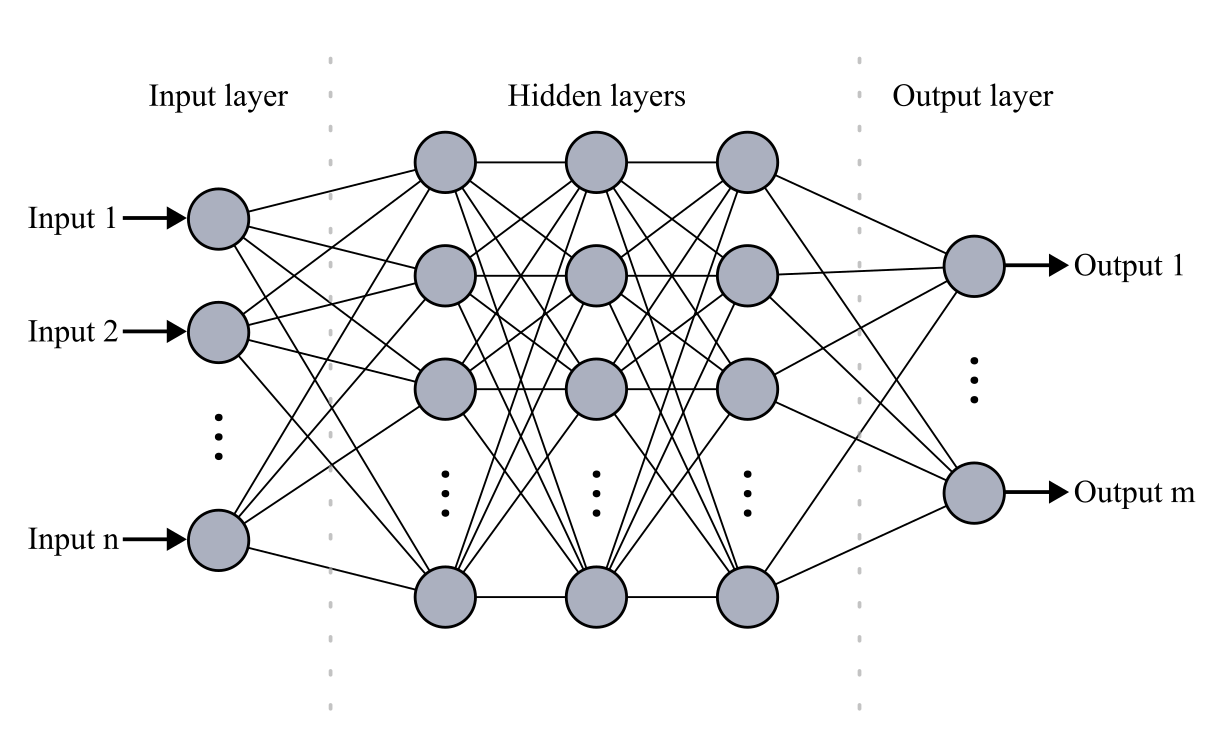
\includegraphics[scale=0.22]{neuralnet.png}
\end{center}
These layers, while visually represented through graphs, are mathematically represented as matrices. In the matrix equation below, we can see a matrix of weights from node $i$ to node $j$ as $w_{i,j}$, a vector of inputs $in_k$, and a vector of outputs produced by multiplying the two, which shows that each output is produced via a combination of each input. \\
\begin{center}
    $\begin{bmatrix}
        w_{1,a} & w_{2,a} & w_{3,a} \\ 
        w_{1,b} & w_{2,b} & w_{3,b} \\ 
        w_{1,c} & w_{2,c} & w_{3,c} \\ 
        w_{1,d} & w_{2,d} & w_{3,d} \\ 
    \end{bmatrix}\begin{bmatrix}
        in_1 \\ in_2 \\ in_3
    \end{bmatrix} = \begin{bmatrix}
        w_{1,a}in_1+w_{2,a}in_2+w_{3,a}in_3 \\
        w_{1,b}in_1+w_{2,b}in_2+w_{3,b}in_3 \\
        w_{1,c}in_1+w_{2,c}in_2+w_{3,c}in_3 \\
        w_{1,d}in_1+w_{2,d}in_2+w_{3,d}in_3
    \end{bmatrix}$
\end{center}

\section{Convolutional Neural Networks}
Convolutional neural networks (or "CNNs") are a variant of neural networks that take 2-dimentional input matrices and use convolutions as layers. 
\subsection{Convolutions}
Convolutions are a matrix operation that "slide" a matrix over another (larger) matrix, performing a dot product for each sub-matrix. For example, a common "sharpening" convolution is shown below.
\begin{center}
    $\begin{bmatrix}
        14 & 26 & 70 & 58 & 19 \\
        36 & 63 & 98 & 99 & 65 \\
        12 & 42 & 86 & 77 & 67 \\
        48 & 22 & 25 & 98 & 100 \\
        22 & 26 & 65 & 52 & 38
    \end{bmatrix}\ast\begin{bmatrix}
        0 & -1 & 0 \\
        -1 & 5 & -1 \\
        0 & -1 & 0
    \end{bmatrix}=\begin{bmatrix}
        113 & 172 & 197 \\
        27 & 146 & 35 \\
        -31 & -146 & 236
    \end{bmatrix}$
\end{center}
To understand what's going on here, let's see where the $113$ came from. 
\begin{center}
    $\begin{bmatrix}
        \color{magenta}14 & \color{magenta}26 & \color{magenta}70 & 58 & 19 \\
        \color{magenta}36 & \color{magenta}63 & \color{magenta}98 & 99 & 65 \\
        \color{magenta}12 & \color{magenta}42 & \color{magenta}86 & 77 & 67 \\
        48 & 22 & 25 & 98 & 100 \\
        22 & 26 & 65 & 52 & 38
    \end{bmatrix}\ast\begin{bmatrix}
        0 & -1 & 0 \\
        -1 & 5 & -1 \\
        0 & -1 & 0
    \end{bmatrix}=\begin{bmatrix}
        \color{magenta}113 & 172 & 197 \\
        27 & 146 & 35 \\
        -31 & -146 & 236
    \end{bmatrix}$
\end{center}
The coloured entries in the first matrix are treated as a seperate matrix. Then, we take the dot product of that matrix and the second matrix, or the "kernel" matrix. (which has no relation to the nullspace kernel!) Now, we can see that that $113$ entry is actually $(0*14)+(-1*26)+(0*70)+(-1*36)+(5*63)+(-1*98)+(0*12)+(-1*42)+(0*86)$. To get second entry in our output, the $172$, we simply shift our pink zone to the left, losing the $\begin{bmatrix}
    13 \\ 36 \\ 12
\end{bmatrix}$ column on the left and gaining the $\begin{bmatrix}
    58 \\ 99 \\ 77
\end{bmatrix}$ column on the right. The reason this particular convolution is a "sharpening" convolution (or more specifically, this kernel is a "sharpening" kernel), is because, when applied to an image, we get this effect:\\
% source: https://setosa.io/ev/image-kernels/
\begin{center}
    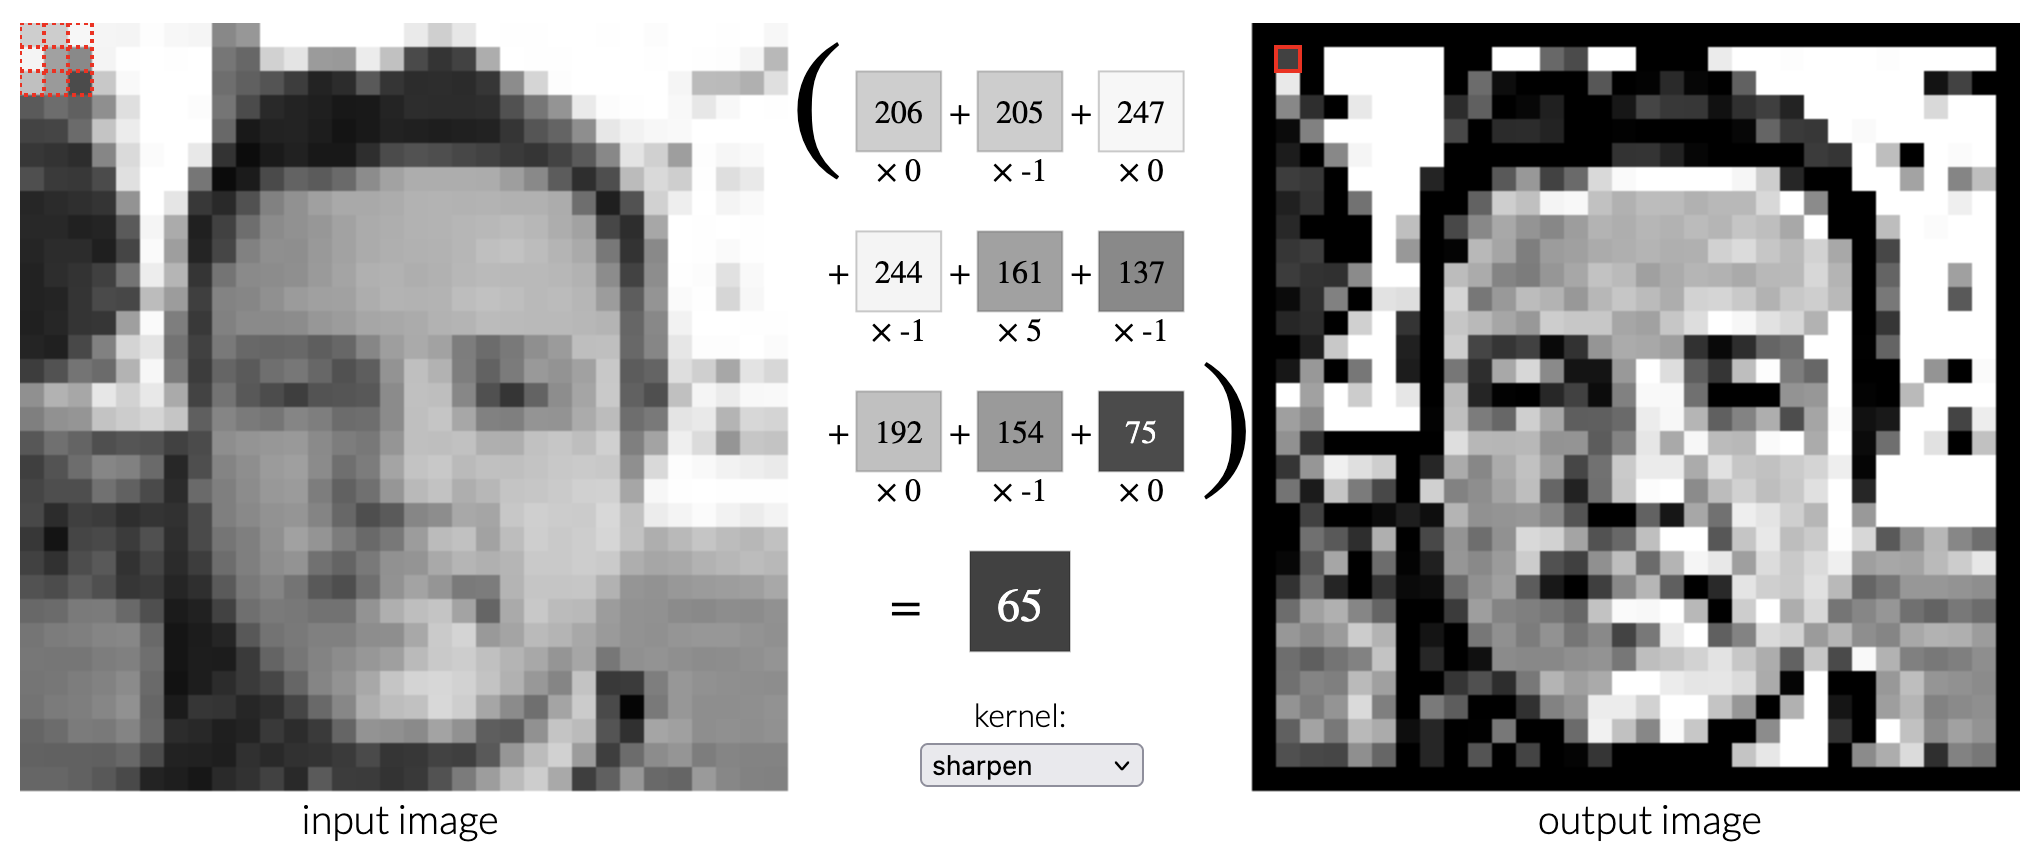
\includegraphics[scale=0.22]{sharpen.png}\\
    Image from: https://setosa.io/ev/image-kernels/
\end{center}
\subsection{CNNs}
Clearly, convolutions can be quite helpful for image processing through filters such as the sharpening filter, Gaussian blur, edge detection, and so much more, but how does this help neural networks? Well, now, when making layers in our neural networks, we initialize kernels of random values and "train" these values to be more helpful. For the purpose of this introduction, we will gloss over what training entails. In a perfect world where neural networks' inner workings were easier to understand, we might actually understand what each of these kernels is doing, but since we do not live in such a world, we'll have to settle for a toy example. Let's say we're building a neural network to detect vertical lines in images. One kernel may end up training to look similar to a vertical sobel filter, which looks like this:\\
\begin{center}
    $\begin{bmatrix}
        1 & 0 & -1 \\
        2 & 0 & -2 \\
        1 & 0 & -1
    \end{bmatrix}$
\end{center}
This kernel, when applied to the same image shown before, does this:
\begin{center}
    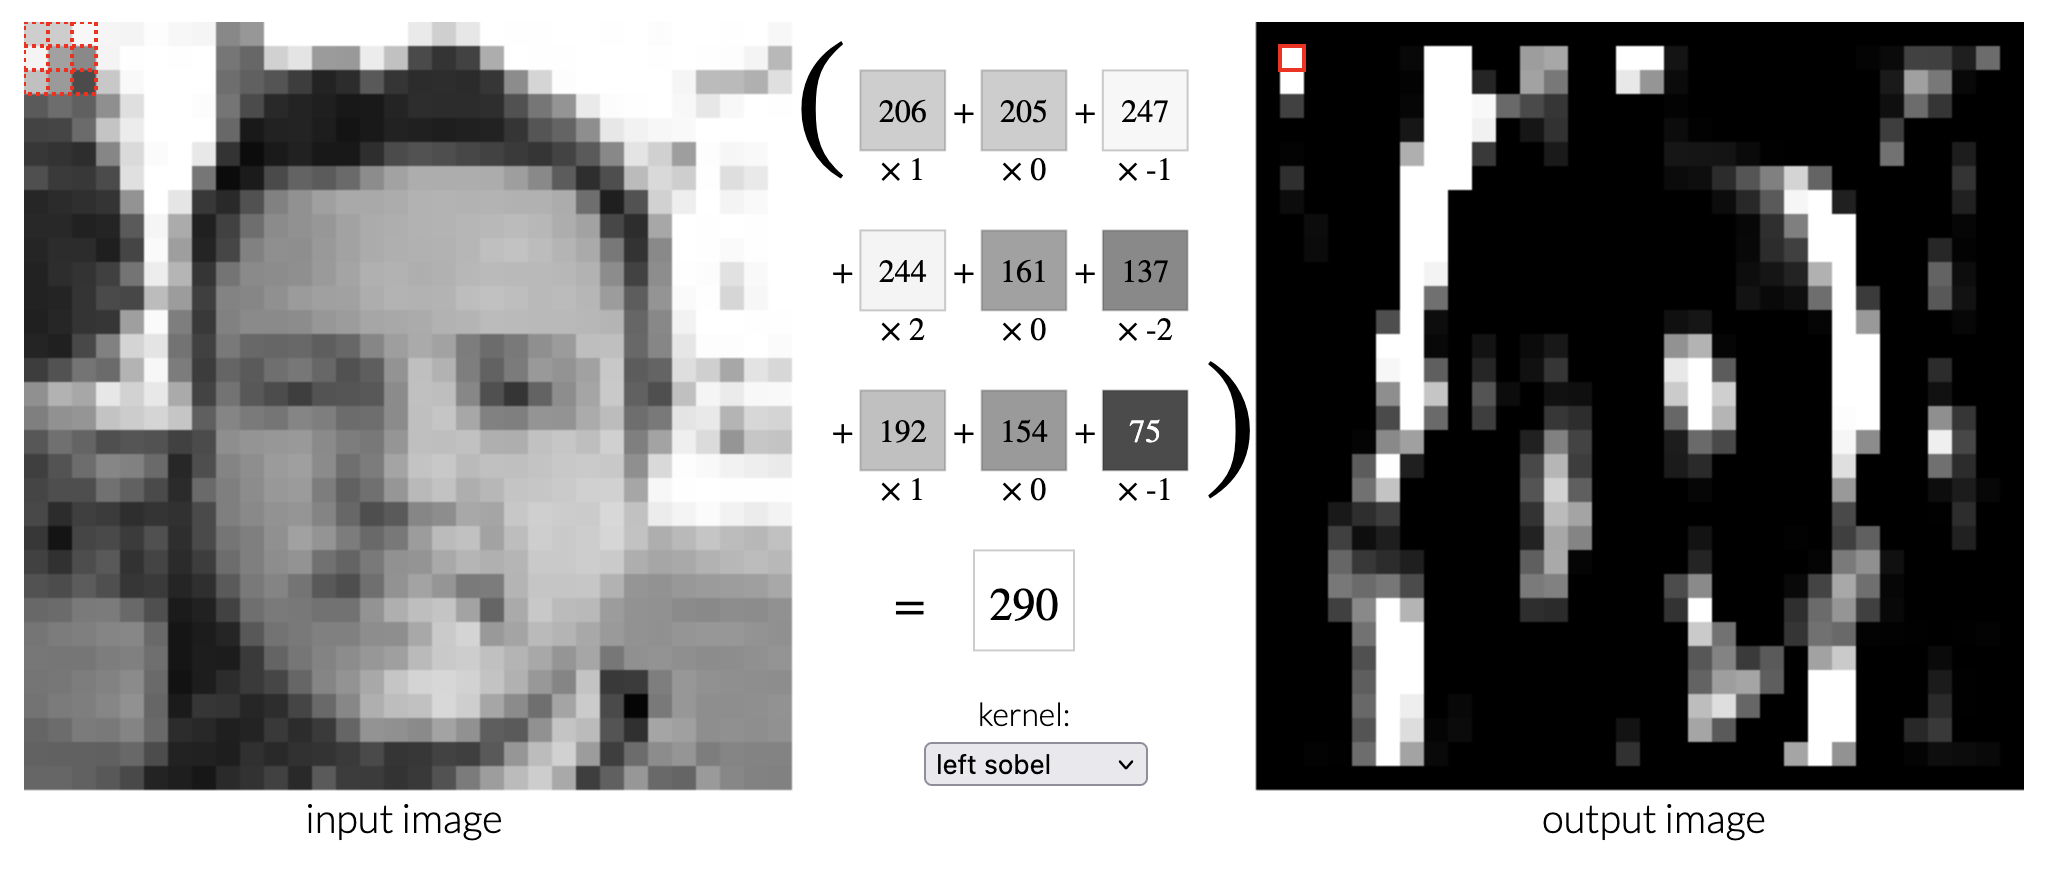
\includegraphics[scale=0.22]{sobel.png}\\
    Image from: https://setosa.io/ev/image-kernels/
\end{center}
As you can see, this kernel "looks for" vertical lines in an image. With this more refined information, a CNN may more easily be able to process this data and tell us whether an image has a vertical line within it or not. Of course, in the real world, our demands of neural networks are a lot more complicated. For example, a common introductory problem for CNNs is classifying the MNIST Dataset of handwritten numbers. This will require more complicated and more numerous kernels to accomplish, but the principle is the same. 
\section{Conclusion}
The big takeaway I would like to leave from this document is that ultimately, neural networks are just thousands of matrix multiplications under the surface. These matrix multiplications, when performed with proper techniques, give rise to algorithms that can drive cars, identify objects, and even generate novel images from text input! The applications for matrices is practically limitless, as Neural Networks are just one of the many practical uses for them.
\end{document}

%TODO: SVD AND PRINCIPLE COMPONENT ANALYSIS
